% Add these to your preamble:
% \usepackage{graphicx}
% \usepackage{booktabs}
% \usepackage{subcaption}
%
% If you copy figures into a dedicated folder, you can also use:
% \graphicspath{{figures/}}

% --- Figure: HS bounds (before vs after) ---
\begin{figure}[ht!]
\centering
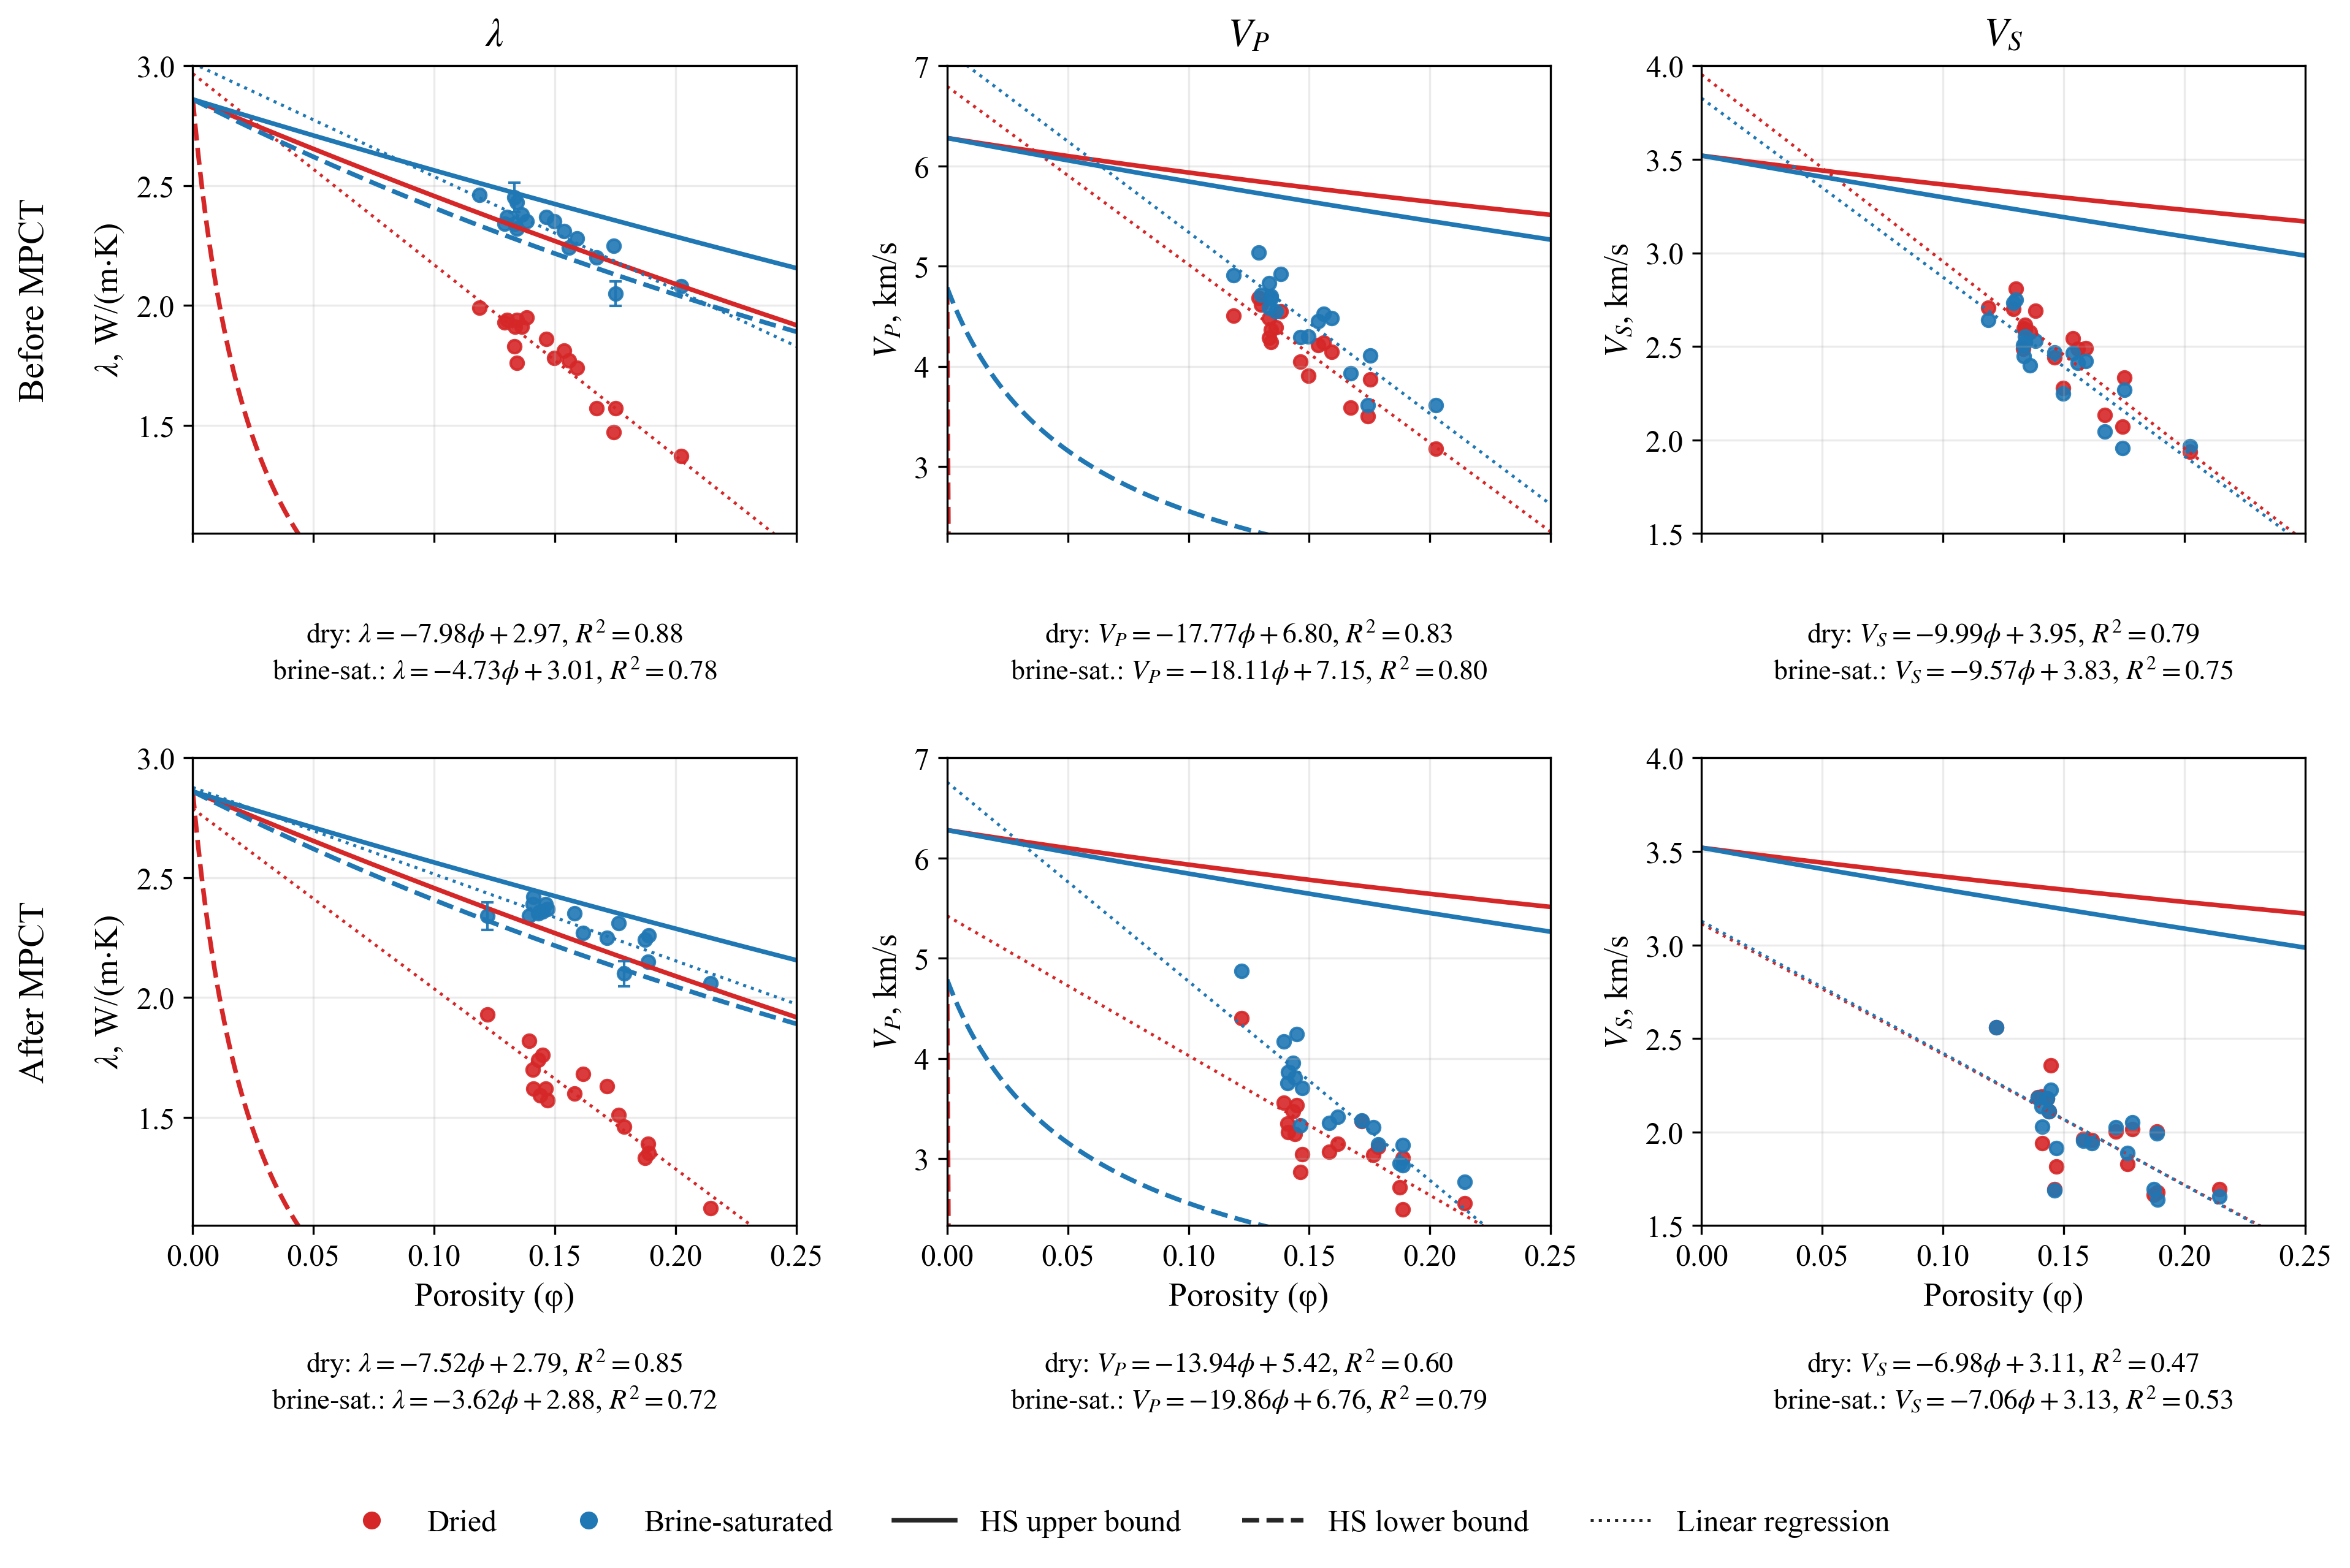
\includegraphics[width=\textwidth]{test_new/porosity_relationships/hs_bounds/hs_bounds_tc_vp_vs_before_after.png}
\caption{HS bounds and linear regression trends for thermal conductivity and elastic velocities versus porosity, shown for dried and brine-saturated samples before and after MPCT. Error bars indicate measurement uncertainty (TC: 2.5\%, $V_P,V_S$: 5\%) for points close to HS bounds.}
\label{fig:hs_bounds_before_after}
\end{figure}

% --- Table: probability-weighted 95% intervals (P2) ---
\begin{table}[ht!]
\centering
\caption{Probability-weighted 95\% intervals for matrix parameters from the HS feasibility model.}
\label{tab:hs_prob_weighted_95ci}
\begin{tabular}{lrrrl}
\toprule
\textbf{Parameter} & \textbf{2.5\%} & \textbf{Median} & \textbf{97.5\%} & \textbf{Units} \\
\midrule
$\lambda_M$ & 2.82 & 2.86 & 2.90 & W/(m$\cdot$K) \\
$V_{P,M}$ & 5621 & 6430 & 7120 & m/s \\
$V_{S,M}$ & 3157 & 3543 & 3916 & m/s \\
\bottomrule
\end{tabular}
\end{table}



% --- Figure: probability-weighted 2D contours (P2) ---
\begin{figure}[ht!]
\centering
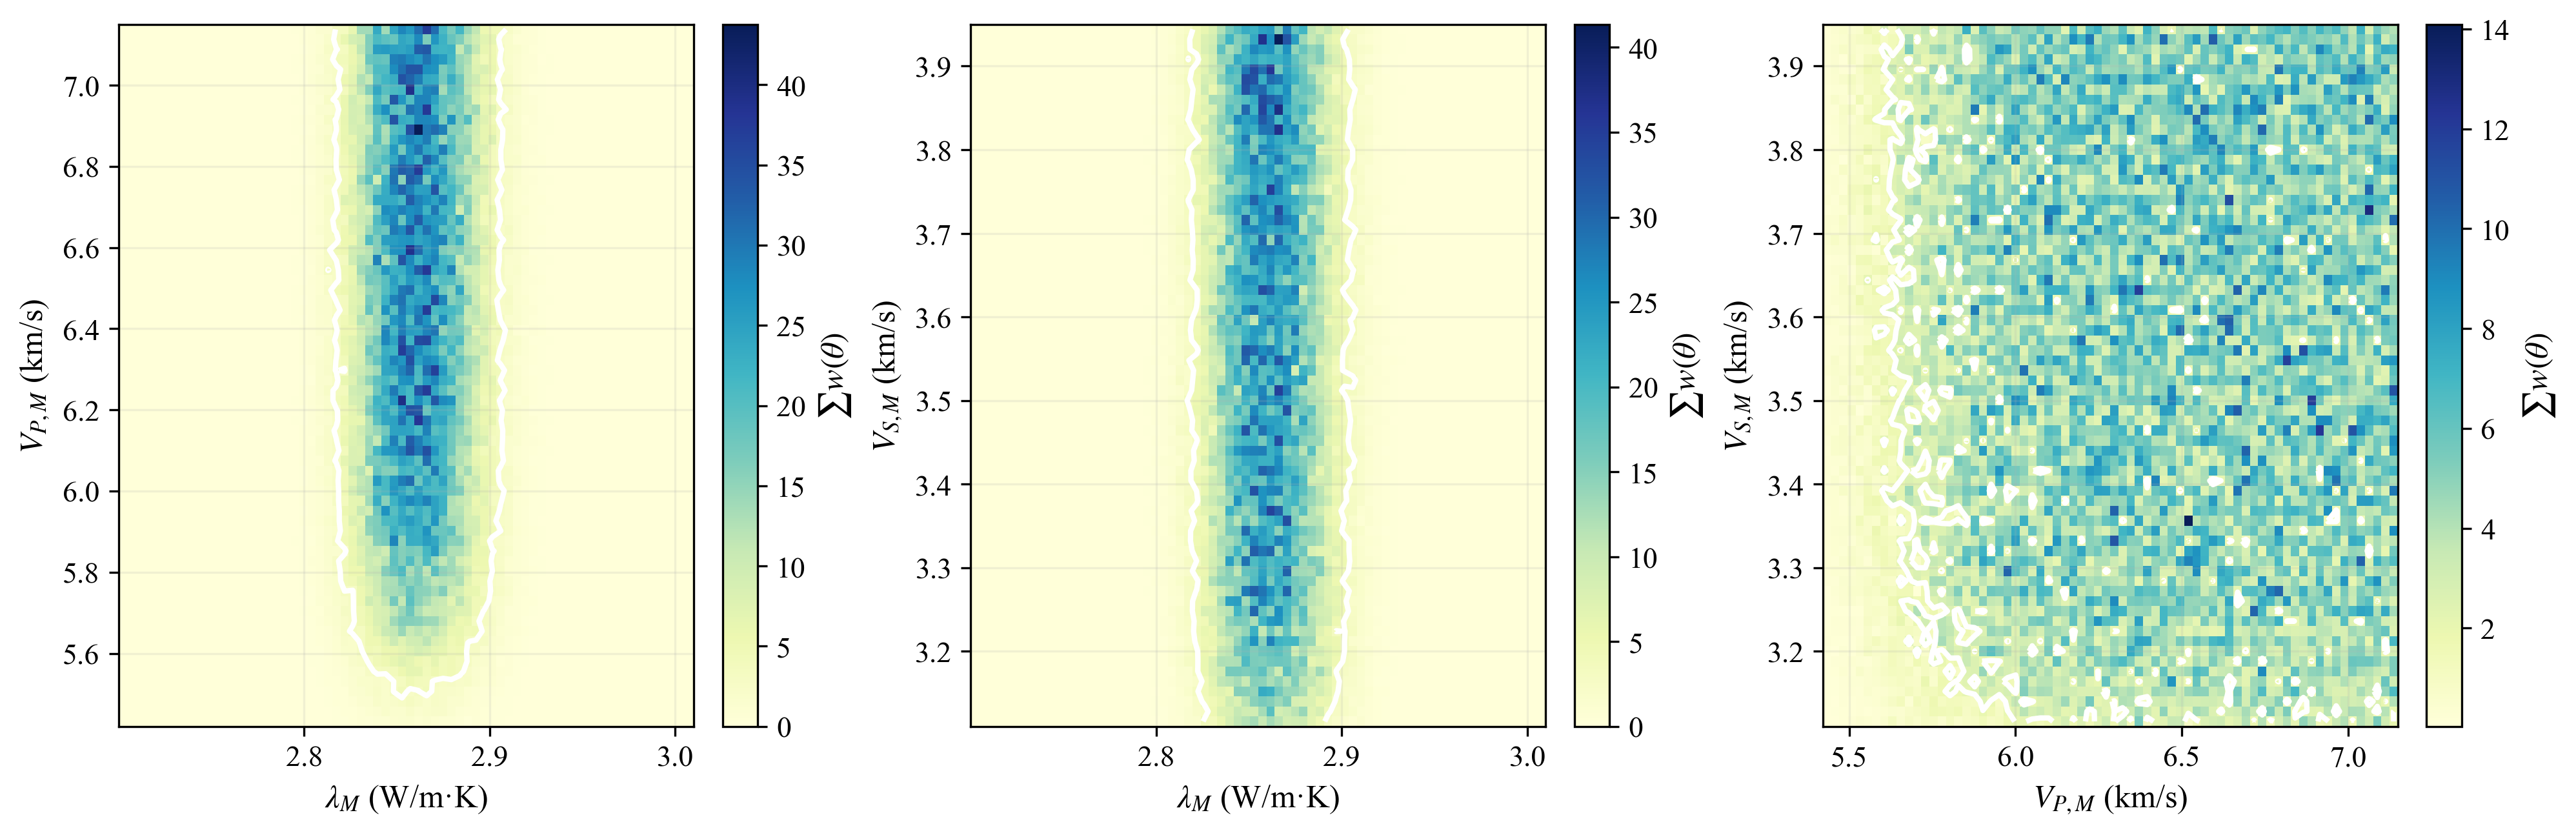
\includegraphics[width=\textwidth]{test_new/hs_matrix_feasible_set/probability_weighted_2d_contours.pdf}
\caption{Probability-weighted 2D contours (95\% mass) for matrix parameters $\lambda_M$, $V_{P,M}$, and $V_{S,M}$ based on the feasibility probability $P(\text{data in HS}\mid\theta)$ under Gaussian measurement errors.}
\label{fig:hs_prob_weighted_2d}
\end{figure}

